\section{Results}
\label{sec:results}

\begin{figure}
\centering
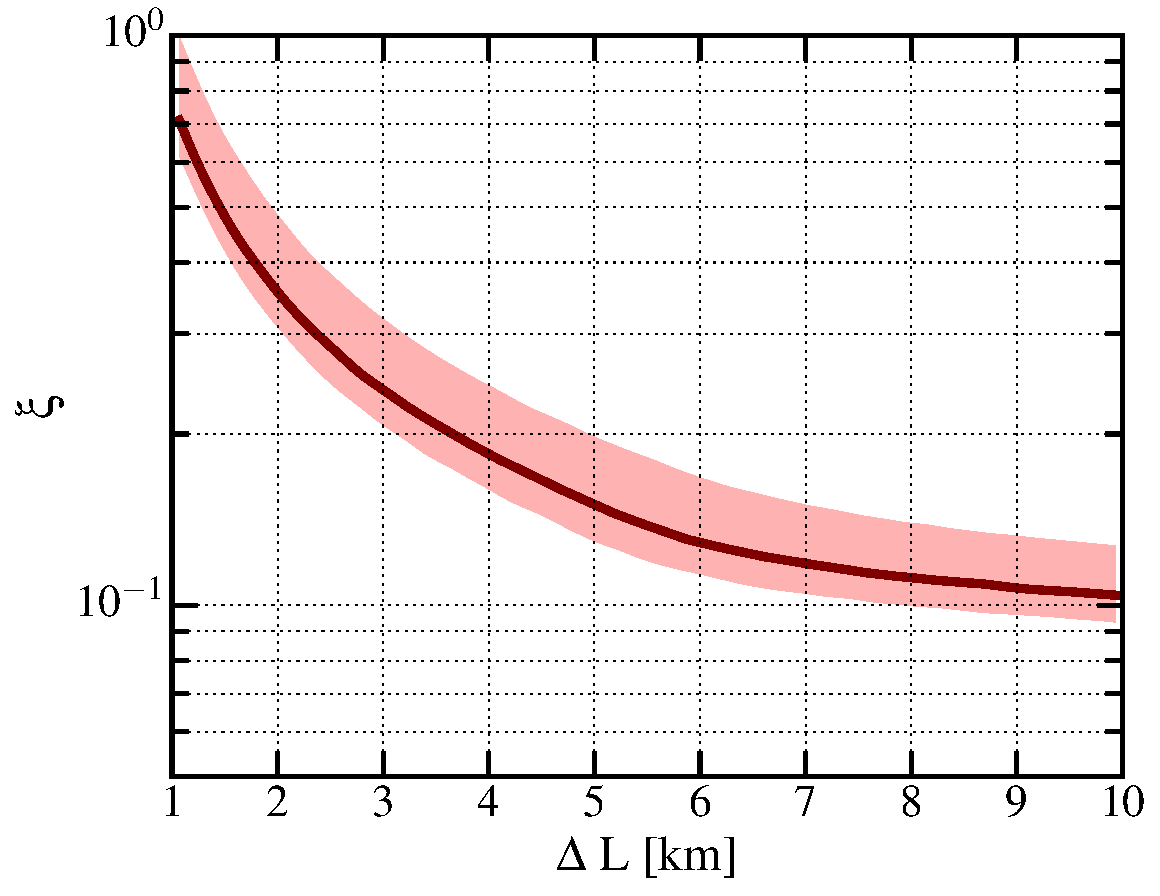
\includegraphics[width=.35\textwidth,keepaspectratio=true]{xi_vs_deltas.pdf}
\caption{FFTT sensitivity to distinguishing saturated case from no magnetic field (upper panel), as a function of maximum array baseline, assuming a survey size of 1 sr, for survey duration of 2 years.\label{fig:sigma_vs_deltas}}
\end{figure}
\begin{figure}
\centering
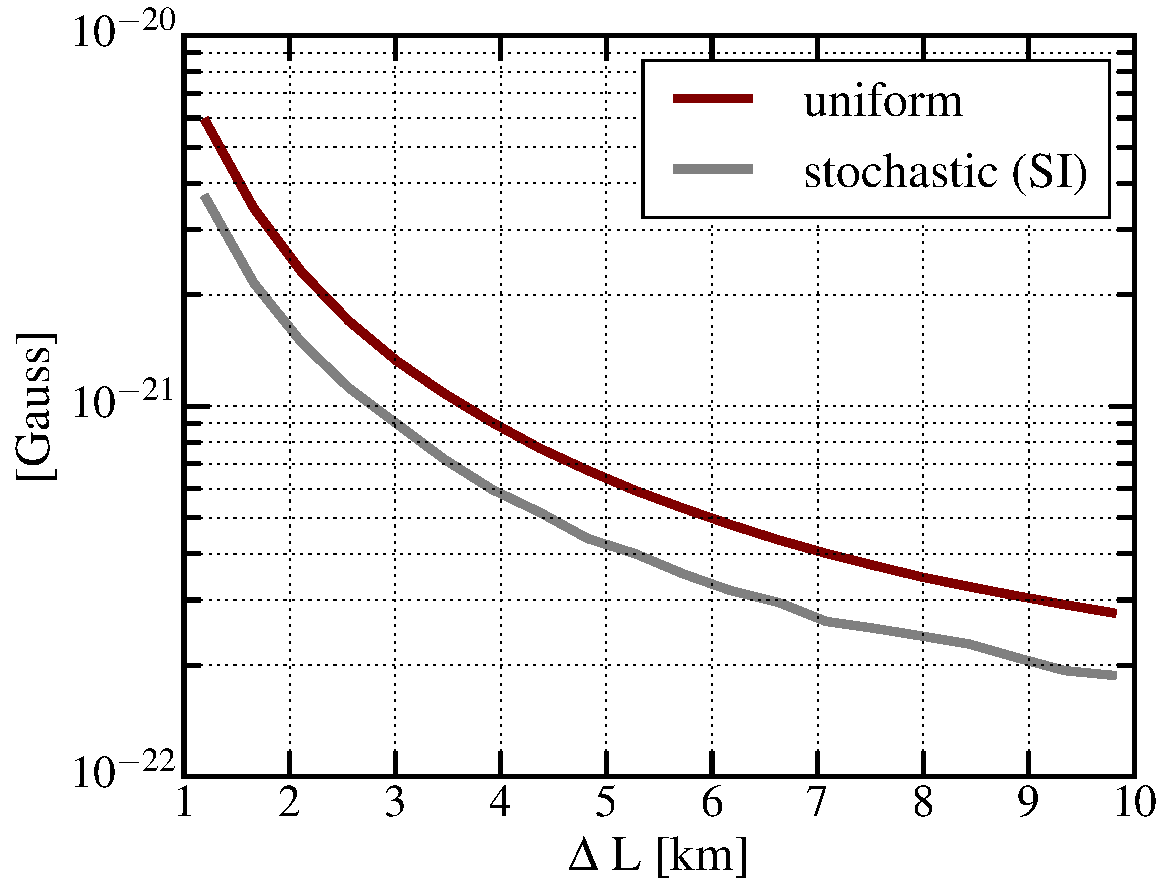
\includegraphics[width=.35\textwidth,keepaspectratio=true]{sigma_vs_deltas.pdf}
\caption{FFTT sensitivity to detecting a uniform and stochastic magnetic field (stochastic field is assumed to have a scale-independent power spectrum), as a function of maximum array baseline, assuming a survey size of 1 sr, for survey duration of 2 years.\label{fig:sigma_vs_deltas}}
\end{figure}

We analyzed sensitivity of an FFTT setup with a total collecting area of $(\Delta L)^2$=4 km$^2$, $\Omega_\text{survey}=1$sr, $t_\text{obs}$=2 year, assuming the array observed redshifts in the range $z\in [15,35]$. Figure \ref{fig:sigma_vs_deltas} shows how this sensitivity changes as a function of the maximum baseline.
\begin{figure}
\centering
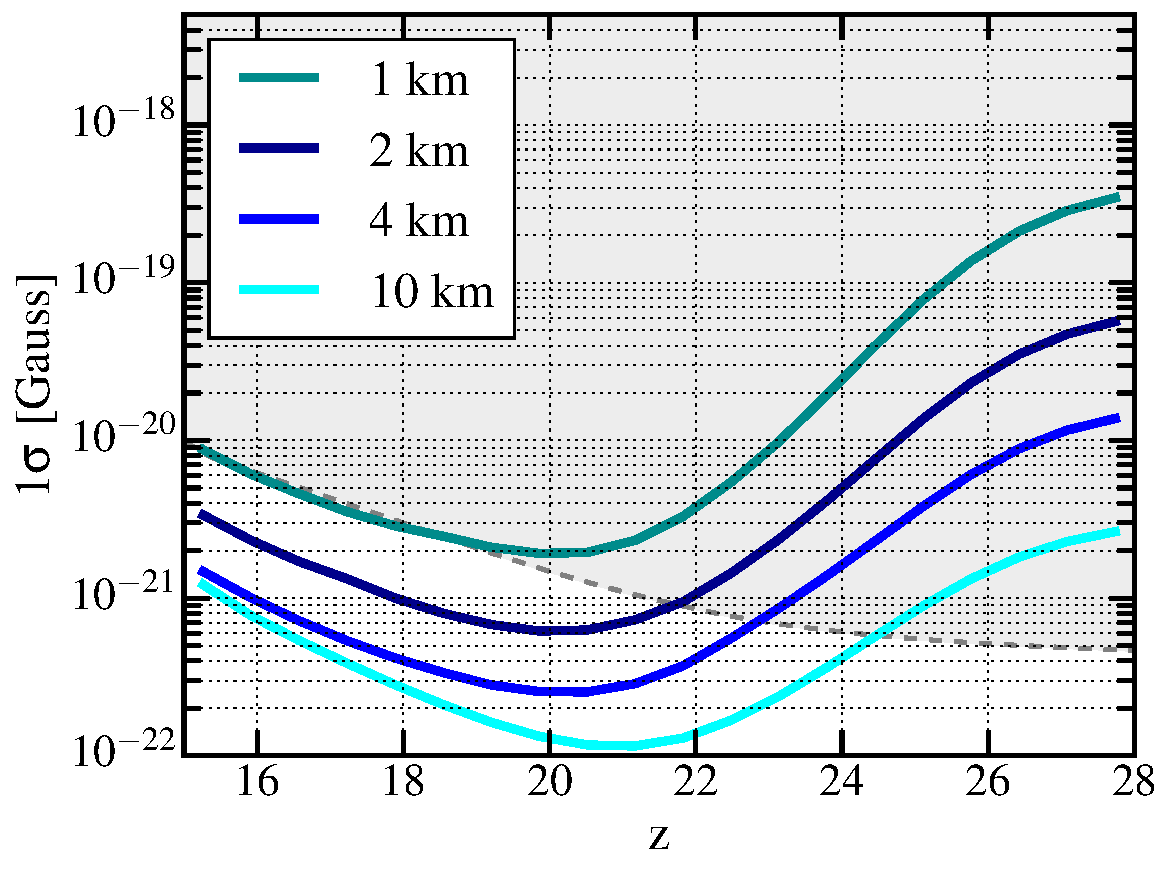
\includegraphics[width=.35\textwidth,keepaspectratio=true]{sigmaB0_vs_z.pdf}
\caption{Saturation ceiling is shown as a shaded gray area, and integrand of \eq{\ref{eq:fisher_patch}} (inverse sqare root of it) is shown as a function of redshift, for several maximum baseline sizes.  When the colored curves are below the saturation limit around their minima, the analysis assuming unsaturated regime is valid.\label{fig:Bsat}}
\end{figure}
\begin{figure}
\centering
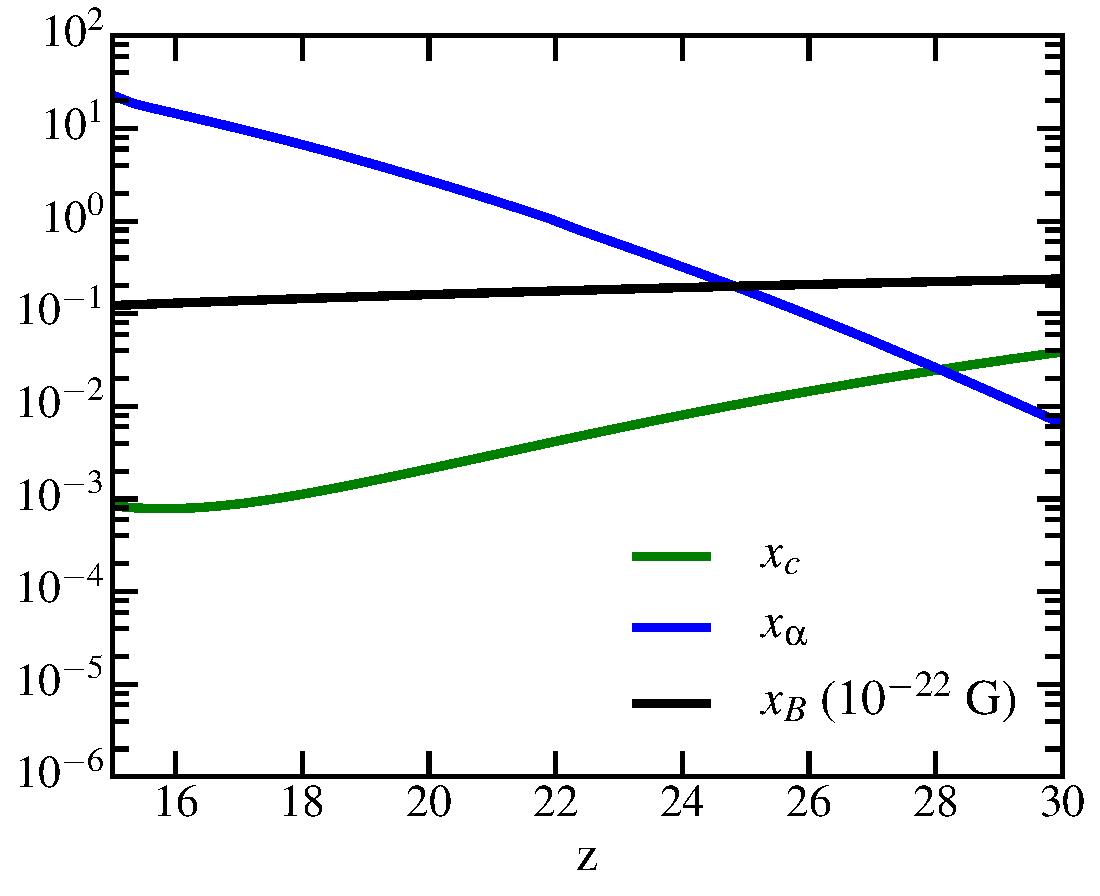
\includegraphics[width=.35\textwidth,keepaspectratio=true]{xs.pdf}
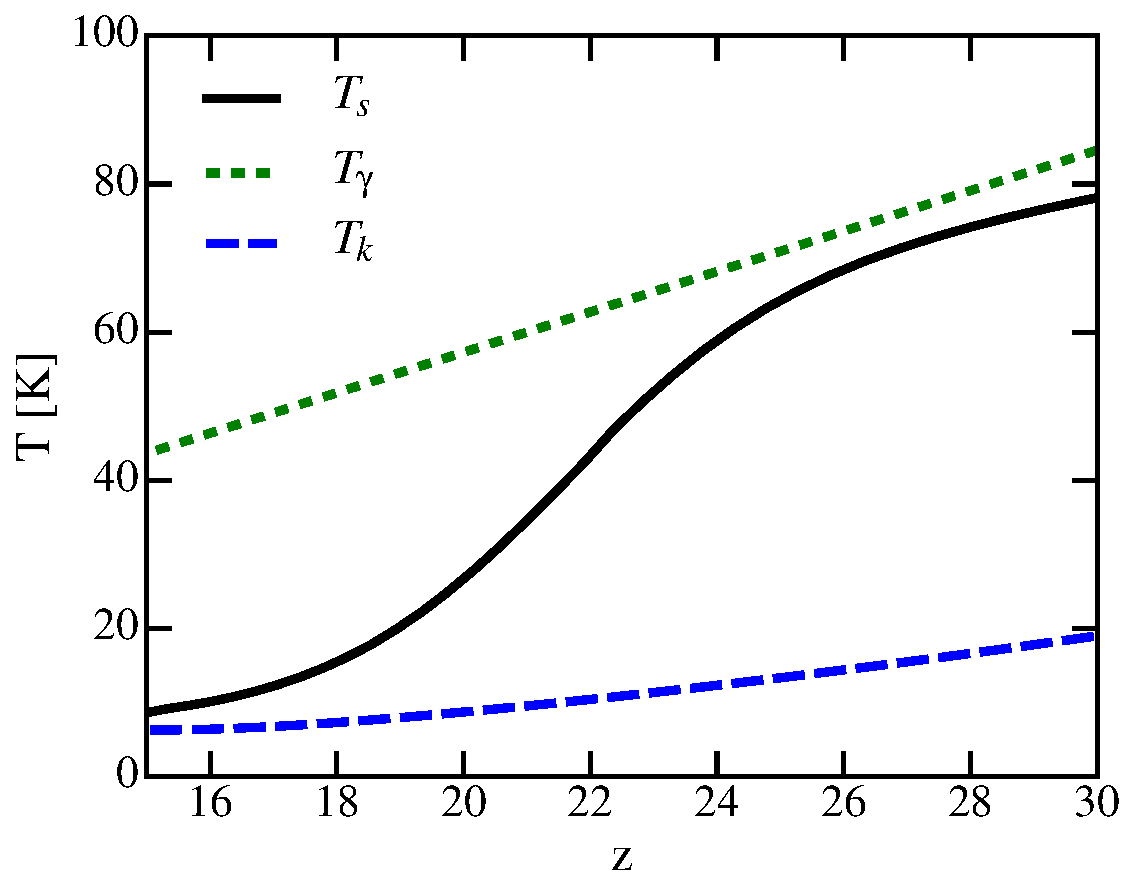
\includegraphics[width=.35\textwidth,keepaspectratio=true]{Ts.pdf}
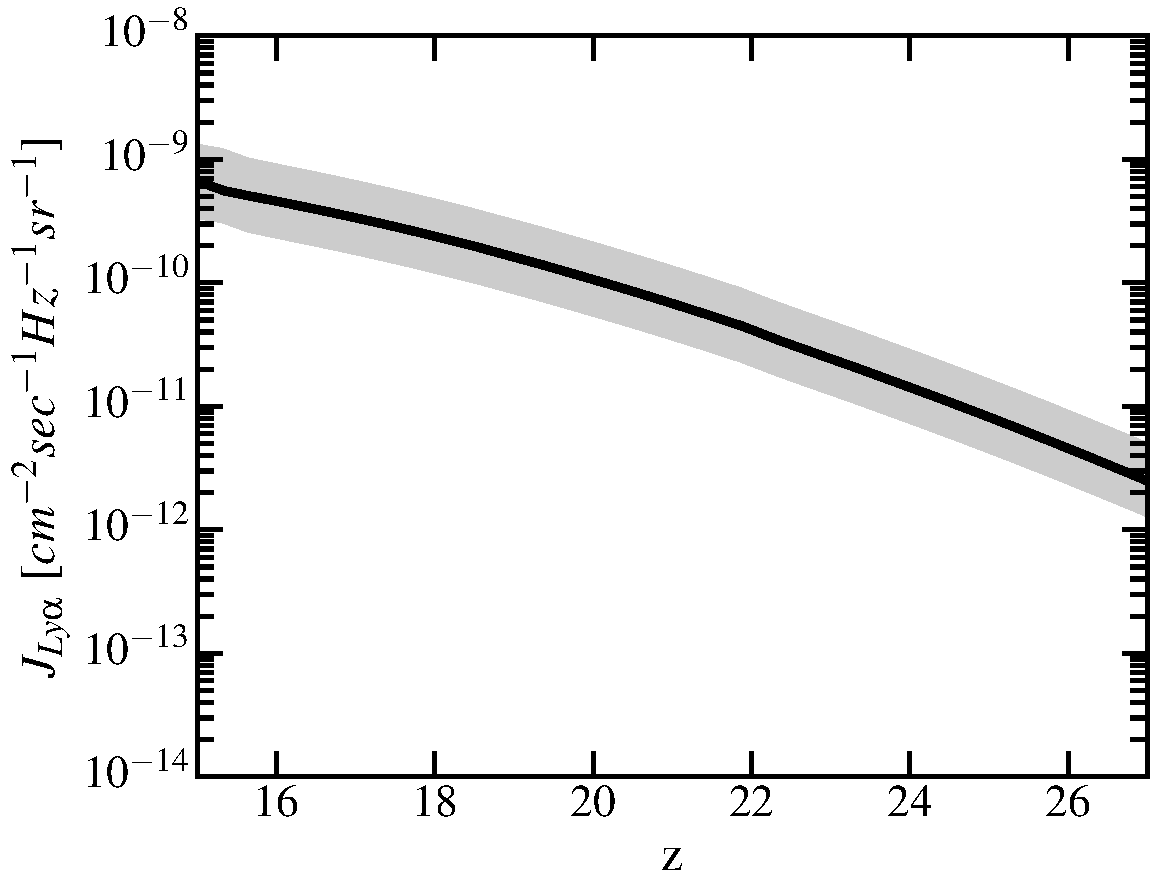
\includegraphics[width=.35\textwidth,keepaspectratio=true]{Jlya.pdf}
\caption{Inputs for sensitivity calculations...\label{fig:cosmo}}
\end{figure}